\section{Optimization}

\setlength{\parskip}{0.7em}
\setlength{\parindent}{0pt}

We formulate surveillance planning as a two-stage mixed-integer optimization model in Pyomo \cite{pyomo_github}. The model jointly decides asset placement across candidate sites, cell coverage, responder assignment, and optional waterhole interventions.

The current scenario optimizes over cars, drones, and cameras with caps
\[
\bar{x}^{\mathrm{car}} = 100,
\qquad
\bar{x}^{\mathrm{drone}} = 3,
\qquad
\bar{x}^{\mathrm{cam}} = 20,
\]
and an annualized scenario budget of
\[
B = 2{,}542{,}700 \text{ USD},
\]
a top-down proxy derived from the 2025/26 Namibia environment vote \cite{namibian2025budget}. Annualized asset and intervention costs are based on the project source inventory \cite{meft_fire_strategy,dji_matrice4_release,reconyx_hyperfire4k,reconyx_cellplan,meft_boreholes_2025}.
The frontier is solved at $\alpha \in \{1.00,\;0.95,\;0.90\}$, and the recommended point is $\alpha = 0.95$.

\subsection{Parameter Values}

\cref{tab:optimization_constants} lists the planning constants used in the current scenario. All costs are annualized USD. Where a direct annual figure was unavailable, capital cost was amortized over the assumed useful life (5 years for vehicles, drones, and cameras; 10 years for borehole infrastructure). Exchange rates use the 2026 USD/NAD market rate of approximately 17.01.

\begin{table}[H]
\centering
\small
\begin{tabular}{llrl}
\hline
\textbf{Parameter} & \textbf{Units} & \textbf{Value} & \textbf{Source} \\
\hline
\multicolumn{4}{l}{\textit{Budget}} \\
Scenario budget $B$ & USD/yr & 2{,}542{,}700 & \cite{namibian2025budget} \\[3pt]
\multicolumn{4}{l}{\textit{Asset costs (annualized)}} \\
Car unit cost $c_{\mathrm{car}}$ & USD/yr & 7{,}810 & \cite{pupkewitz_hilux} \\
Drone unit cost $c_{\mathrm{drone}}$ & USD/yr & 1{,}580 & \cite{dji_matrice4_store} \\
Camera unit cost $c_{\mathrm{cam}}$ & USD/yr & 160 & \cite{reconyx_hyperfire4k,reconyx_cellplan} \\
Intervention capital $K_w$ & USD/yr & 4{,}150 & \cite{meft_boreholes_2025} \\
Intervention tourism penalty $T_w$ & USD/yr & 400 & assumption \\[3pt]
\multicolumn{4}{l}{\textit{Asset caps and baselines}} \\
Car cap $\bar{x}^{\mathrm{car}}$ & units & 100 & scenario choice \\
Car included baseline $\underline{x}_{\mathrm{car}}$ & units & 100 & scenario choice \\
Drone cap $\bar{x}^{\mathrm{drone}}$ & units & 3 & scenario choice \\
Camera cap $\bar{x}^{\mathrm{cam}}$ & units & 20 & scenario choice \\
Camera bundle size $m^{\mathrm{cam}}$ & units/site & 5 & \cite{nwr_live_camera} \\[3pt]
\multicolumn{4}{l}{\textit{Mobility}} \\
Car response speed & km/h & 28 & assumption \\
Drone response speed & km/h & 55 & \cite{dji_matrice4_specs} \\
Car coverage radius & m & 7{,}000 & assumption \\
Drone coverage radius & m & 12{,}000 & assumption \\
Camera detection radius & m & 75 & \cite{reconyx_hyperfire4k} \\
Dummy fallback time $\tau^{\mathrm{dummy}}$ & min & 225 & assumption \\[3pt]
\multicolumn{4}{l}{\textit{Wildfire penalty}} \\
Fire threshold $\tau^{\mathrm{fire}}$ & min & 45 & assumption \\
Fire penalty slope $\beta^{\mathrm{fire}}$ & --- & 0.09 & assumption \\
Fire penalty weight $\lambda^{\mathrm{fire}}$ & --- & 2.5 & assumption \\[3pt]
\multicolumn{4}{l}{\textit{Protection and intervention effects}} \\
Protection leverage scale & --- & 1.0 & assumption \\
Camera gain factor & --- & 0.5 & assumption \\
Camera risk suppression & --- & 0.35 & assumption \\
Waterhole dispersion benefit & --- & 0.15 & assumption \\
Waterhole influence radius & m & 5{,}000 & assumption \\
\hline
\end{tabular}
\caption{Planning constants for the current optimization scenario. ``Assumption'' denotes a calibrated model parameter without direct external source.}
\label{tab:optimization_constants}
\end{table}

\subsection{Model Structure}

The model is built on linked sets of candidate sites $\mathcal{S}$, landscape cells $\mathcal{C}$, asset types $\mathcal{A}$, response arcs $\mathcal{R}$, waterhole interventions $\mathcal{W}$, and fire-delay breakpoints $\mathcal{B}$. Each response arc $r \in \mathcal{R}$ links one site to one cell with a feasible responder type and a travel time. Each cell carries a base protection value $p_c$, a composite risk weight $\rho_c$, and a wildfire risk weight $\phi_c$.

Coverage and intervention effects are precomputed. Camera lockdowns and waterhole interventions contribute marginal gains $g^{\mathrm{cam}}_{c,s}$ and $g^{\mathrm{int}}_{c,w}$ respectively.

The key decision variables are integer deployment counts $x_{sa}$ for each site--asset pair, binary site and asset activation flags, binary cell coverage and response-arc assignment indicators, realized response times $t_c$, piecewise-linear wildfire penalty variables, and binary intervention selections $q_w$ and camera lockdown decisions $\ell_s$.

\subsection{Constraints}

\subsubsection{Camera Bundles}

Cameras are deployed as fixed-size bundles at eligible waterhole sites:
\[
x_{s,\mathrm{cam}} = m^{\mathrm{cam}} \,\ell_s,
\qquad
\forall s \in \mathcal{S}^{\mathrm{waterhole}},
\]
where $m^{\mathrm{cam}}$ is the bundle size. This is consistent with the current Etosha live-camera deployment model \cite{nwr_live_camera,reconyx_hyperfire4k}.

\subsubsection{Budget}

The model charges only for asset units above an included baseline $\underline{x}_a$. With $e_a = \max(0, \sum_s x_{sa} - \underline{x}_a)$ representing the chargeable excess, the budget constraint is
\[
\sum_{a \in \mathcal{A}} c_a e_a
+ \sum_{s \in \mathcal{S}} F_s v_s
+ \sum_{w \in \mathcal{W}} K_w q_w
\le B,
\]
where $c_a$ is the annualized unit cost, $F_s$ is site activation cost, and $K_w$ is intervention capital cost.

\subsubsection{Coverage and Response}

A cell can only be covered if at least one feasible site--asset pair is active. Each cell receives exactly one response: either a real arc or a dummy fallback at $\tau^{\mathrm{dummy}} = 225$ minutes. The realized response time is
\[
t_c = \sum_{r \in \mathcal{R}(c)} \tau_r z_r + \tau^{\mathrm{dummy}} d_c.
\]

\subsubsection{Wildfire Penalty}

Wildfire penalty is interpolated via a convex combination over precomputed breakpoints:
\[
f_c = \sum_{b \in \mathcal{B}} \pi_b \lambda_{cb},
\qquad
\sum_{b} \lambda_{cb} = 1,
\quad
\lambda_{cb} \ge 0,
\]
where $\pi_b$ is the penalty at breakpoint $b$. These breakpoint penalties are generated from a bounded fire-delay curve rather than chosen arbitrarily. For a breakpoint response time $\tau_b$, the penalty is zero up to the fire threshold $\tau^{\mathrm{fire}}$, then grows approximately exponentially with slope $\beta^{\mathrm{fire}}$, and finally saturates at a plateau. In symbols, the breakpoint values are constructed from a bounded version of
\[
\pi(\tau_b) \approx \exp\!\Bigl(\beta^{\mathrm{fire}} \min\{\tau_b-\tau^{\mathrm{fire}},\,60\}\Bigr) - 1,
\]
with the rise smoothed and capped so that the penalty does not increase without bound at extreme response times. The interpolation variables $\lambda_{cb}$ then let the optimizer represent the wildfire penalty for each realized response time $t_c$ with a linear formulation.

\subsection{Objective Functions}

The protection objective sums base coverage rewards, camera gains at locked-down waterholes, and intervention gains:
\[
P
=
\sum_c p_c y_c
+
\sum_c \sum_s g^{\mathrm{cam}}_{c,s}\,\ell_s
+
\sum_c \sum_w g^{\mathrm{int}}_{c,w}\,q_w.
\]
The first term rewards ordinary binary coverage: if cell $c$ is covered, the model earns its precomputed base protection value $p_c$; otherwise it earns zero from that term. The second term adds the marginal protection gain from camera lockdowns. Each coefficient $g^{\mathrm{cam}}_{c,s}$ is precomputed from the waterhole-camera geometry and risk layer, so activating lockdown $\ell_s = 1$ contributes that gain to every cell influenced by site $s$. The third term works the same way for waterhole interventions: if intervention $w$ is selected, the model receives the precomputed gain $g^{\mathrm{int}}_{c,w}$ in each affected cell.

The response objective combines risk-weighted travel time, wildfire delay penalty, and tourism costs from interventions:
\[
R
=
\sum_c \rho_c t_c
+
\lambda^{\mathrm{fire}} \sum_c \phi_c f_c
+
\sum_w T_w q_w,
\]
where $\lambda^{\mathrm{fire}}$ is the configured wildfire weight and $T_w$ is the annual tourism cost of intervention $w$.

Each term has a different mechanism. The travel-time term $\rho_c t_c$ penalizes slow service in proportion to the cell's composite risk weight $\rho_c$: one extra minute in a high-risk cell costs more than one extra minute in a low-risk cell. The realized response time itself is
\[
t_c = \sum_{r \in \mathcal{R}(c)} \tau_r z_r + \tau^{\mathrm{dummy}} d_c,
\]
so the optimizer either pays the travel time of the selected real arc or, if no feasible real arc is chosen, the fallback time $\tau^{\mathrm{dummy}}$.

The wildfire term $\lambda^{\mathrm{fire}} \phi_c f_c$ is layered on top of travel time. Here $\phi_c$ scales the fire exposure of the cell, $\lambda^{\mathrm{fire}}$ controls the global importance of wildfire delay relative to ordinary response time, and $f_c$ is the interpolated value of the bounded fire-delay curve evaluated at $t_c$. Because the breakpoint values $\pi_b$ are generated from the exponential form above, this term is exactly where the model converts long response times into rapidly increasing fire-related penalty until the configured plateau is reached.

The final term $\sum_w T_w q_w$ is different from the first two because it is not cell-specific. It is a direct additive penalty for selecting waterhole intervention $w$, representing annual tourism or visitor-experience cost that the model must trade against the protection benefits of those interventions.

\subsection{Two-Stage Frontier Construction}

Rather than combining protection and response into an arbitrary weighted sum, we use an $\epsilon$-constraint frontier. Stage one solves $\max\;P$ subject to all constraints, yielding $P^{\max}$. Stage two, for each $\alpha$, solves $\min\;R$ subject to the same constraints plus the protection floor $P \ge \alpha P^{\max}$.

\begin{figure}[H]
\centering
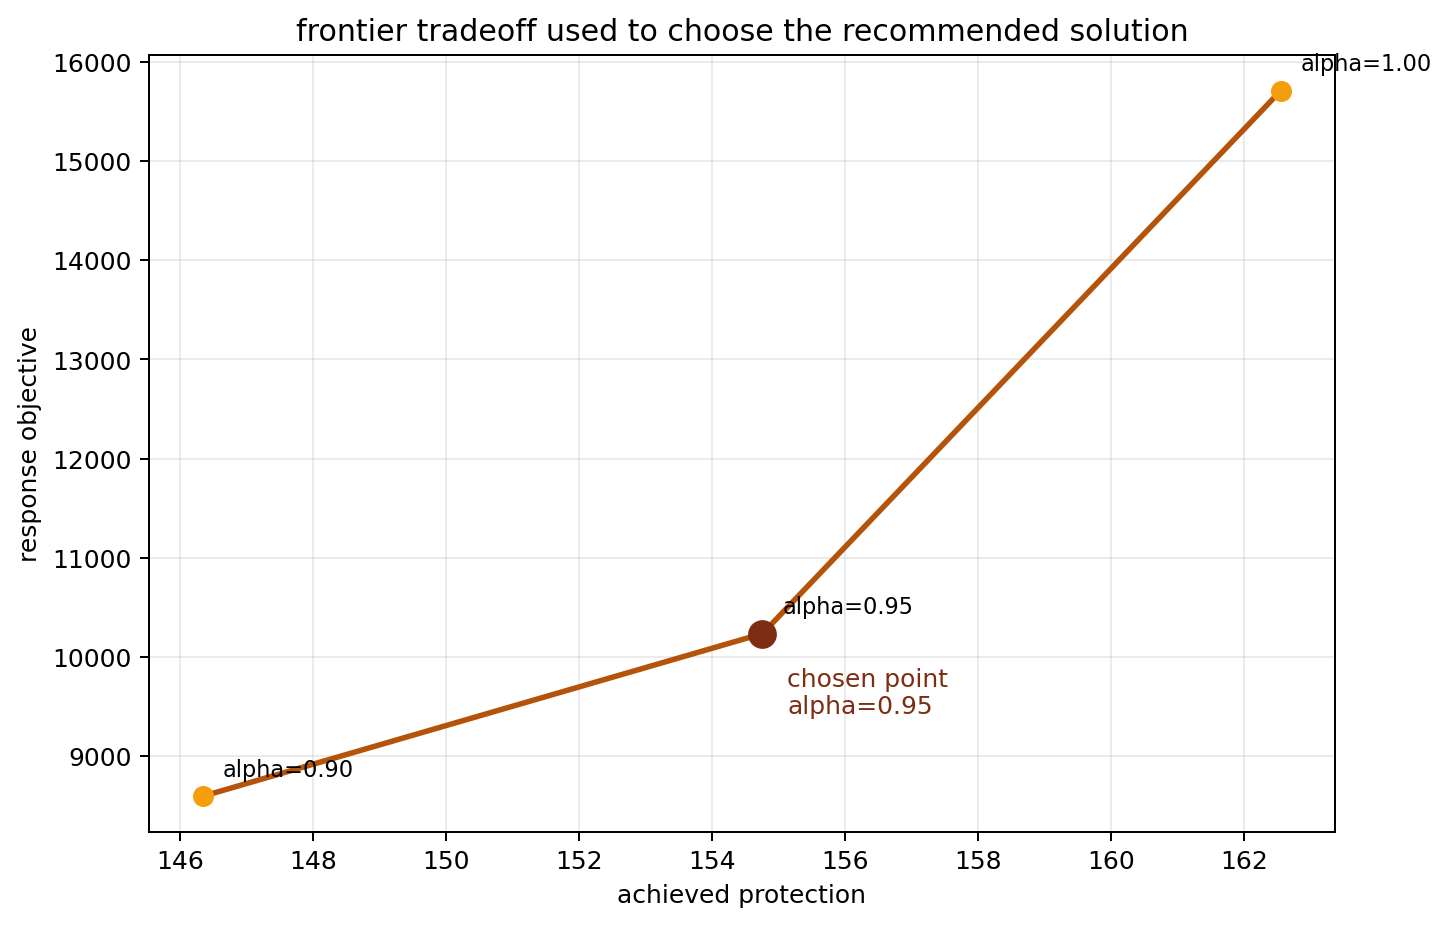
\includegraphics[width=0.8\textwidth]{optimization_components/02_frontier_tradeoff.png}
\caption{Protection--response frontier used to choose the recommended solution}
\label{fig:optimization_frontier_components}
\end{figure}

The current solve gives $P^{\max} = 162.554$. The full frontier is
\[
(\alpha, P, R) \in
\left\{
(1.00,\;162.554,\;15710.593),\;
(0.95,\;154.759,\;10234.513),\;
(0.90,\;146.346,\;8595.114)
\right\}.
\]
The step from $\alpha = 1.00$ to $0.95$ gives a substantial reduction in response cost ($-35\%$) while sacrificing only $5\%$ of protection, so the middle point is used as the recommended solution.

\subsection{Current Resource Mix}

The chosen solution under $\alpha = 0.95$ activates
\[
x^{\star}_{\mathrm{car}} = 100,
\qquad
x^{\star}_{\mathrm{drone}} = 3,
\qquad
x^{\star}_{\mathrm{cam}} = 20.
\]
It also selects
\[
q^{\star} = 3 \text{ interventions},
\qquad
\ell^{\star} = 4 \text{ locked-down waterholes},
\]
across
\[
103 \text{ selected sites.}
\]

The total budget used at the recommended point is
\[
B^{\star} = 26915,
\]
which is far below the current available budget:
\[
B^{\star} \ll B = 2{,}542{,}700.
\]
This means the current solve is primarily cap-constrained rather than budget-constrained.

\begin{figure}[H]
\centering
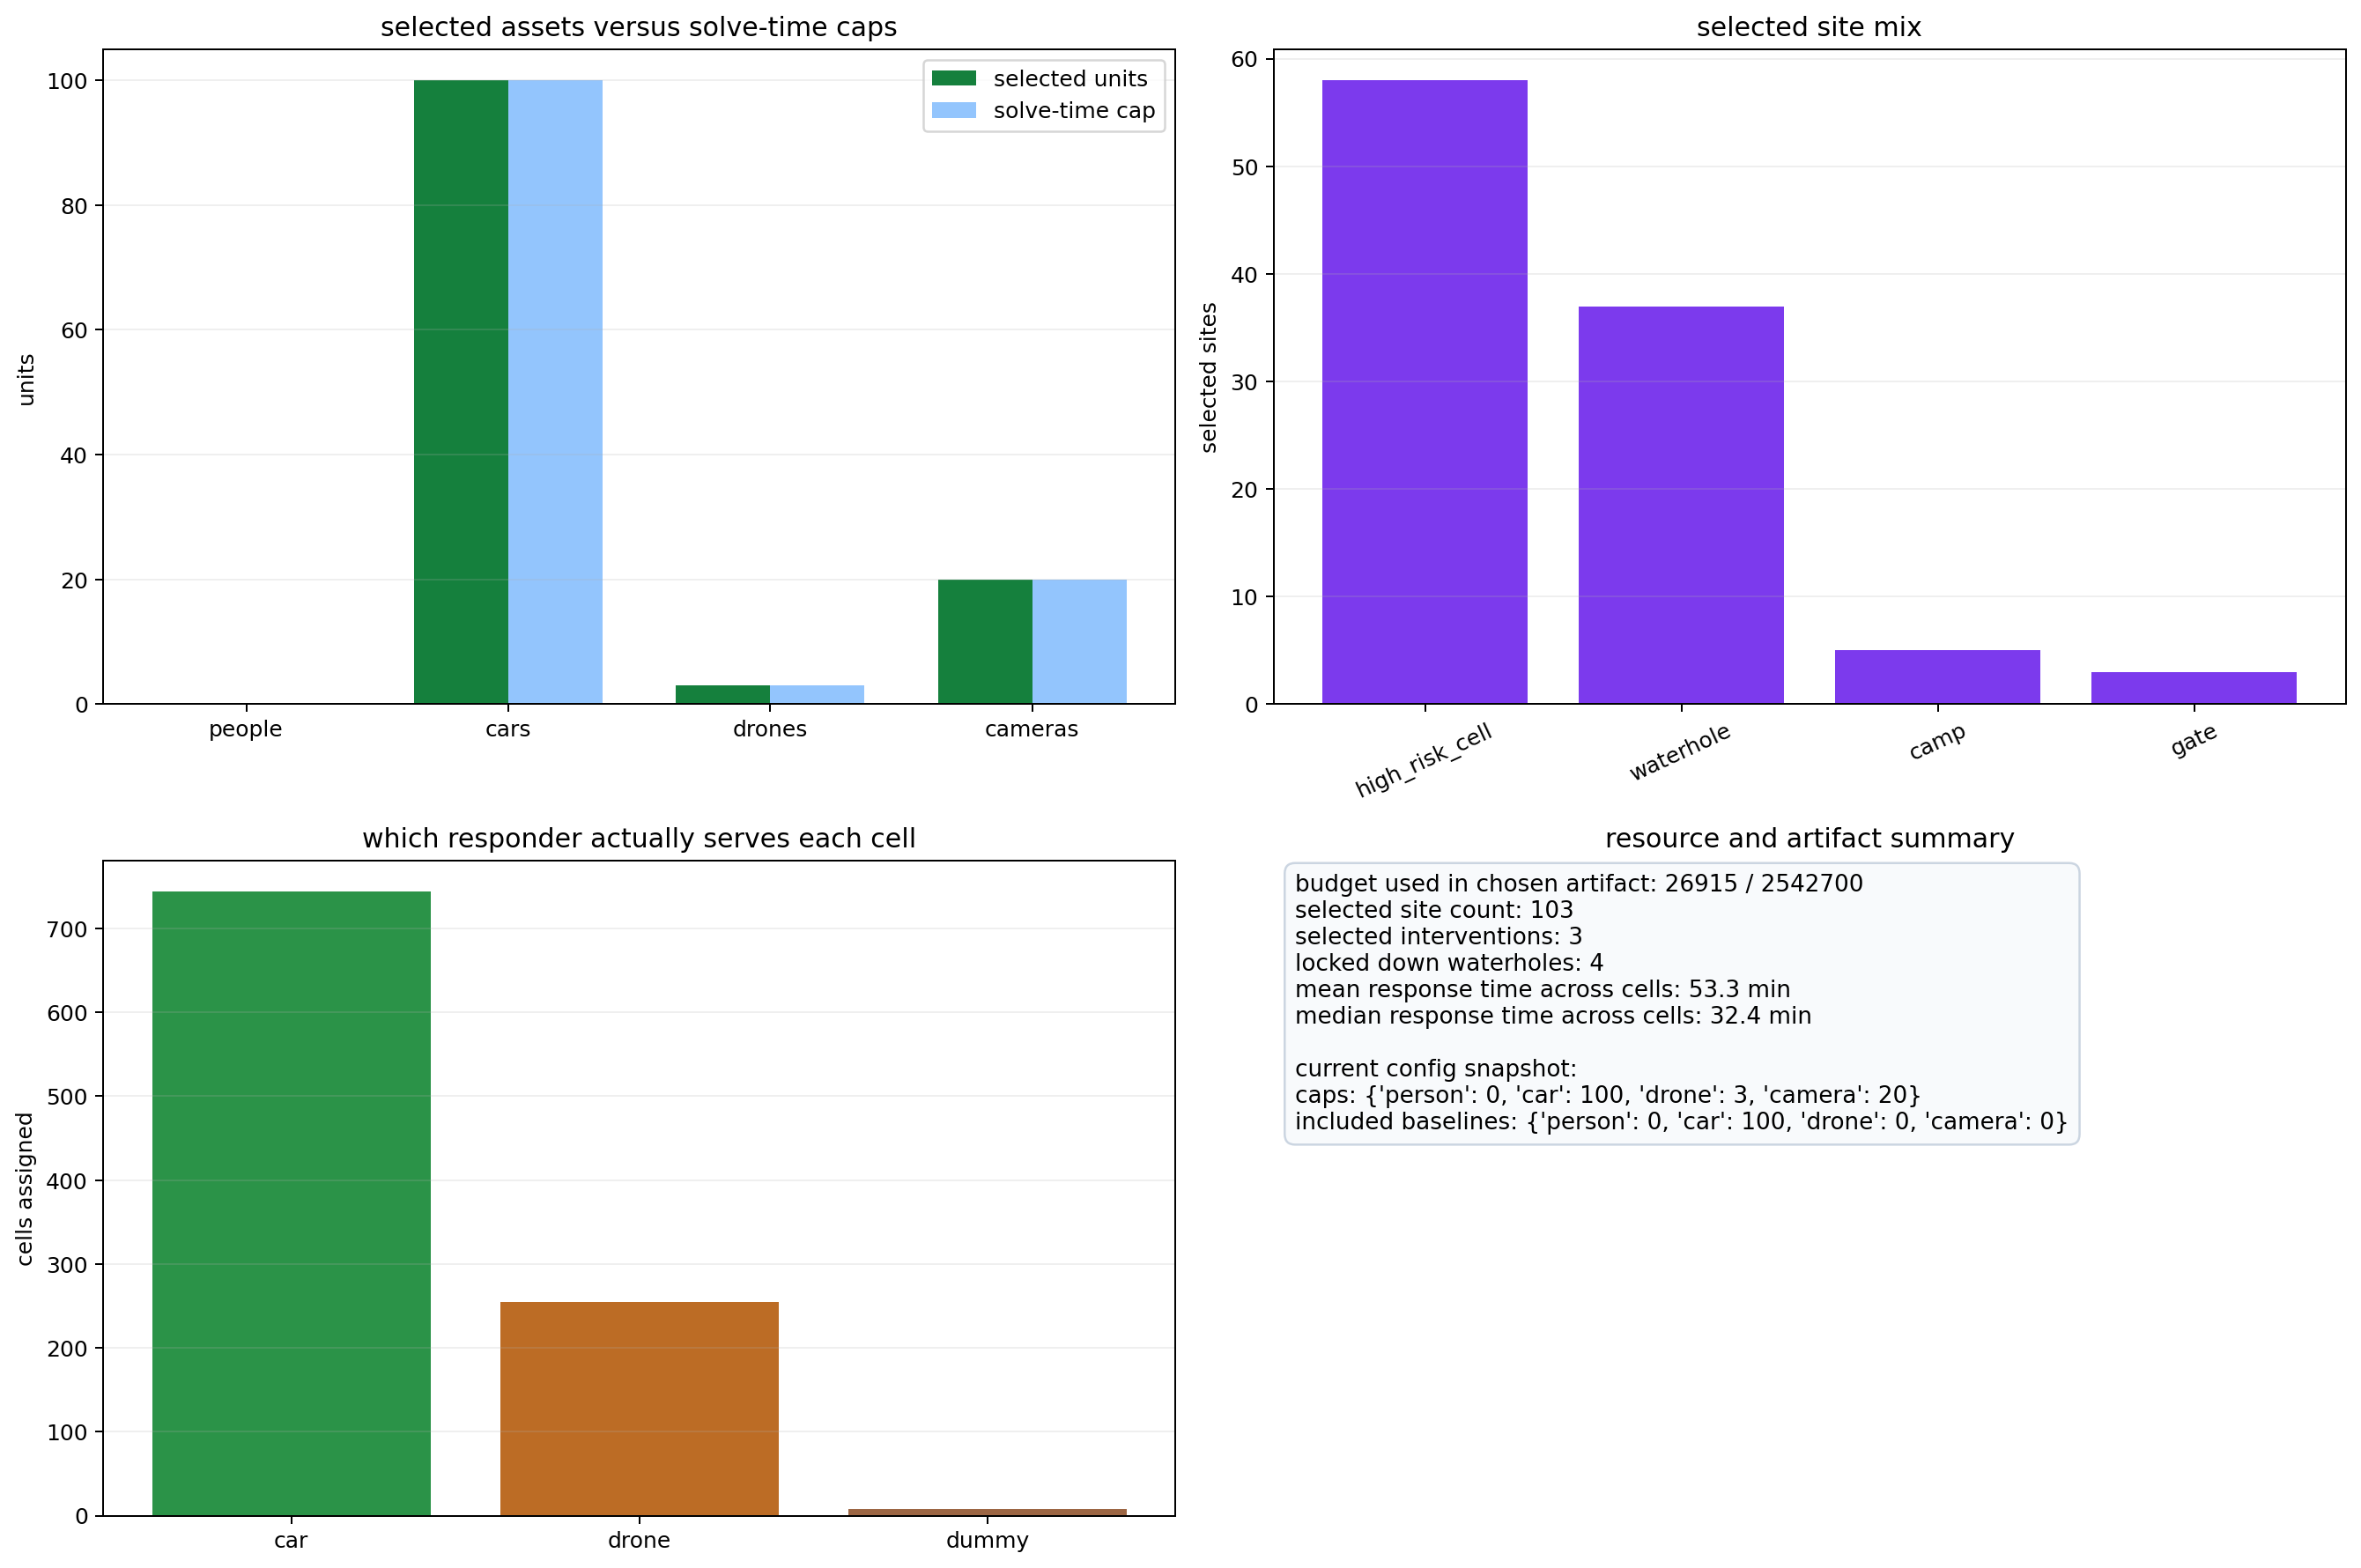
\includegraphics[width=0.95\textwidth]{optimization_components/03_resource_summary.png}
\caption{Selected asset counts versus caps and the resulting site mix}
\label{fig:optimization_resource_summary}
\end{figure}

\cref{fig:optimization_resource_summary} shows that the recommended solution saturates all three active asset caps. Cars, drones, and cameras are all used up to their respective limits, which is exactly what we would expect once the scenario budget becomes very large relative to the annualized marginal asset costs.

Here, ``dummy'' does not represent a deployable asset or intervention. It is a per-cell fallback assignment variable used to preserve feasibility when no real response arc is selected. If $d_c = 1$, then the model sets $t_c = \tau^{\mathrm{dummy}} = 225$ minutes for that cell. The dummy therefore has zero direct contribution to the protection objective and no standalone budget cost. Its cost appears only inside the response objective through the terms
\[
\rho_c \tau^{\mathrm{dummy}}
\qquad \text{and} \qquad
\lambda^{\mathrm{fire}} \phi_c f_c(\tau^{\mathrm{dummy}}).
\]
Under the current parameterization, with $\tau^{\mathrm{dummy}} = 225$, $\tau^{\mathrm{fire}} = 45$, $\beta^{\mathrm{fire}} = 0.09$, and $\lambda^{\mathrm{fire}} = 2.5$, the dummy-induced fire penalty reaches the plateau
\[
f_c(225) = \exp\!\bigl(0.09 \cdot 60\bigr) - 1 \approx 220.41,
\]
so the approximate per-cell response cost of assigning the dummy is
\[
R_c^{\mathrm{dummy}}
\approx
225\,\rho_c + 2.5 \cdot 220.41\,\phi_c
=
225\,\rho_c + 551.02\,\phi_c.
\]
If both normalized risk weights were equal to one, one dummy-served cell would contribute about $776$ objective units. In practice, this means the model can tolerate dummy fallback in low-risk cells more easily than in cells with simultaneously high composite risk and high wildfire risk.

\subsection{Spatial Allocation and Response Behavior}

The optimization output is spatial, not only numeric. It tells us which sites were selected, which cells were counted as covered, what response time each cell receives, and which responder type is assigned to each cell.

\begin{figure}[H]
\centering

\includegraphics[width=0.95\textwidth]{optimization_components/04_spatial_solution.png}
\caption{Spatial allocation of selected sites, covered cells, response times, and assigned responders}
\label{fig:optimization_spatial_solution}
\end{figure}

As shown in \cref{fig:optimization_spatial_solution}, the chosen solution distributes cars broadly, uses drones to extend reach into more difficult areas, and uses camera lockdowns around waterholes to raise protection values in place. The response assignment layer also makes clear that the optimization is solving a service problem, not just a siting problem.

The responder breakdown is 744 cells served by car, 255 by drone, and only 8 falling back to the dummy response at $\tau^{\mathrm{dummy}} = 225$ minutes.

\subsection{Cell-Level Interpretation}

The effective protection in each cell is $p^{\mathrm{eff}}_c = p_c + \sum_s g^{\mathrm{cam}}_{c,s}\,\ell_s + \sum_w g^{\mathrm{int}}_{c,w}\,q_w$, and the response burden is $r_c = \rho_c t_c + \lambda^{\mathrm{fire}} \phi_c f_c$. Cells with large risk weight or long response time dominate the response objective; cells near selected waterholes gain the most from camera and intervention effects.

\begin{figure}[H]
\centering

\includegraphics[width=0.95\textwidth]{optimization_components/05_cell_metrics.png}
\caption{Cell-level diagnostics for response time, protection gain, and objective behavior}
\label{fig:optimization_cell_metrics}
\end{figure}

\cref{fig:optimization_cell_metrics} highlights that the optimization is not simply chasing the highest-risk cells with the nearest asset. Instead, it balances broad coverage, fast response on high-risk cells, fixed and marginal deployment costs, wildfire delay penalties, and the incremental gains from waterhole actions.

For the current artifact, the response-time distribution is
\[
t_c \in
\left[
0.50,\;
225.00
\right],
\]
with empirical quartiles
\[
Q_{0.25} = 15.99,
\qquad
Q_{0.50} = 32.38,
\qquad
Q_{0.75} = 75.12.
\]

\subsection{Interpretation of the Current Solve}

The current optimization output shows three important things.

First, the frontier is real. The model is not solving a single hard-coded asset mix. Lowering $\alpha$ relaxes the protection floor and gives the optimizer room to improve the response objective.

Second, under the current annualized budget proxy, budget is no longer the tight constraint. The model immediately fills the available caps for cars, drones, and cameras. That means the next binding limits are the asset caps and the structure of the intervention and coverage relationships.

Third, the chosen solution remains spatially selective even when the asset counts saturate. The model still has to decide where to place those capped assets and which cells they should actually serve.

Taken together, the optimization stage transforms the risk maps from the previous section into an operational deployment plan. The output is therefore not only a map of danger, but a feasible set of surveillance and intervention decisions that trades off protection and response quality in a transparent, equation-based way.
